% Configuración a 2 columnas

%\documentclass[3p]{elsarticle}
\documentclass[3p,twocolumn]{elsarticle}

% Paquete con el tipo de codificación del lenguaje
\usepackage[utf8]{inputenc}
% Paquete para mostrar el número de líneas
\usepackage[modulo]{lineno}
\linenumbers
% Paquete para mostrar imágenes
\usepackage{graphicx}
\graphicspath{ {/home/acamon/TFG/GitHub/TFG/Recursos/Fotos/} }
% Paquete para resaltar enlaces y referencias
\usepackage{hyperref}
% Configuración del paquete
\hypersetup{
  breaklinks=true,  
  colorlinks=true,
  urlcolor=urlcolor,
  linkcolor=linkcolor,
  citecolor=citecolor,
}
% Modifica el pie de la primera página para poner el número de la misma
\makeatletter
\def\ps@pprintTitle{%
   \let\@oddhead\@empty
   \let\@evenhead\@empty
   \def\@oddfoot{\reset@font\hfil\thepage\hfil}
   \let\@evenfoot\@oddfoot
}
\makeatother
% Paquete para cambiar color texto
\usepackage[dvipsnames]{xcolor}


%====================================================================================================================================================%
%====================================================================================================================================================%


% Inicio del documento
\begin{document}

\title{TFG} % Título del TFG

\author[1]{Aarón Casado Monge} % Autor del TFG
\ead{aaron.casado@uah.es} % Correo del alumno

\author[2]{Juan José Cuadrado Gallego} % Tutor del TFG
\ead{jcg@uah.es} % Correo del profesor

% Dirección de la Escuela Politécnica Superior de UAH
\address{University of Alcala, Polytechnic School, Computer Science Department, Scientific and Technological Campus, Politechnic Building. Office: O243, 28805, Alcala de Henares, Madrid, Spain}

% Abstracto del TFG
\begin{abstract}
Clusterización (qué es y para qué sirve) - Técnicas (para qué sirven) - Paquetes 
\end{abstract}

% Palabras clave del TFG
\begin{keyword}
BigData, Statistics, Bioestatistics, Data Science, Clustering
\end{keyword}

\maketitle % Creación del Título, autores, abstracto...
 
 
%====================================================================================================================================================%
%====================================================================================================================================================%
 
 
% Introducción del TFG
\section{Introducción}

% Intento de poner una foto
%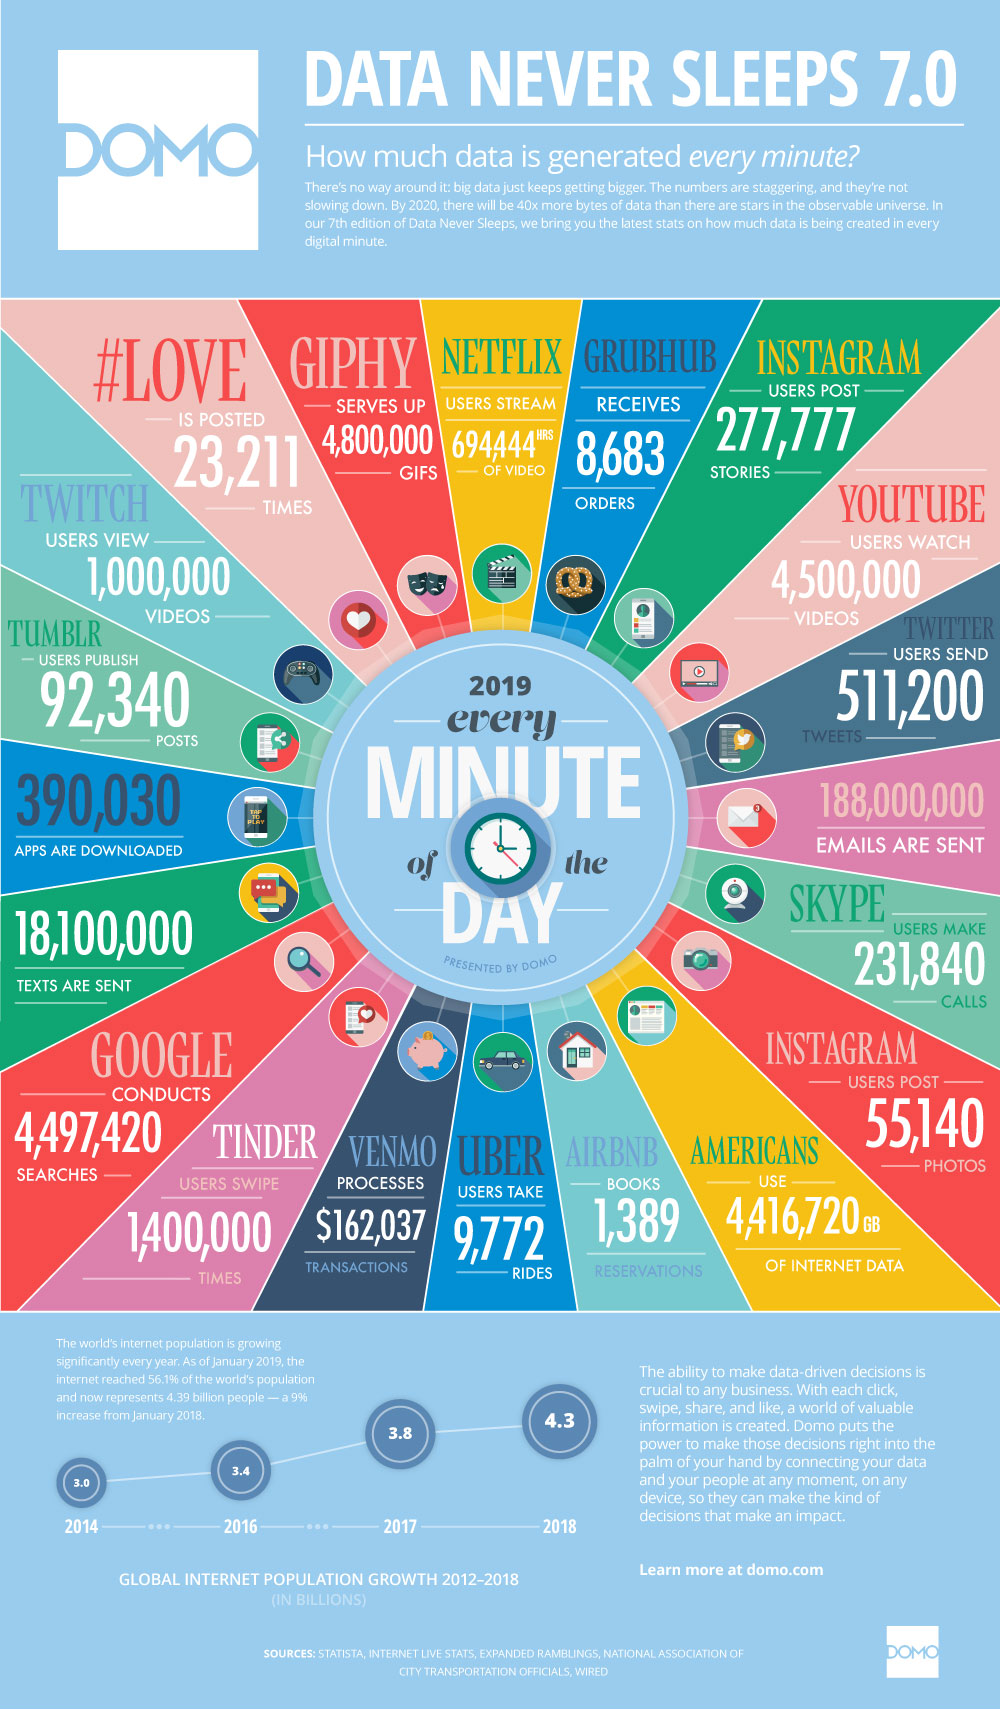
\includegraphics[width=\linewidth]{19_domo_data-never-sleeps-7}

Desde finales del sigo \textsc{xx} se ha considerado que vivimos en la ``era de la información", una etapa caracterizada por el incremento, desarrollo y propagación de emergentes tecnologías de la información y comunicación que han permitido al ser humano romper las barreras de la distancia, el tiempo y el lugar a la hora de comunicarse y compartir información; actividades que han sido decisivas en nuestra historia \cite{cita1}. Sin embargo, la era en la que realmente vivimos es la ``era de los datos"; cada día se generan más de dos mil quinientos millones de petabytes\footnote {Un Petabyte es una unidad de información o almacienamiento de datos equivalente a un cuadrillon de bytes, mil terabytes o un millón de gigabytes. En este caso, es el equivalente a 2.5 quintillones de bytes.} de datos provenientes de comercios, ciencias, Internet y casi cualquier actividad del día a día \cite{cita2} que acaban volcados en redes de ordenadores, sitios web, bases de datos y otros medios de almacenaje. 

Esta explosión de datos, a la que se ha denominado \textbf{Big Data}, se debe al alto grado de computarización de la sociedad y el avance de herramientas de recolección y almacenamiento de datos. Negocios en todo el mundo generan grandes cantidades de datos derivados de transacciones, stock de productos,  platillas de empleados, etc. Las ramas de la ciencia producen datos de manera constante frutos de experimentos, observaciones, recogida de muestras, etc. Y más recientemente, Internet y las redes sociales han sido las principales responsables del aumento excesivo de datos, siendo usadas por millones de personas simultáneamente.

Y, aunque esto ha supuesto una considerable mejora para la humanidad pues la información nunca había sido tan accesible, también ha traido consecuencias negativas y problemas, como el almacenamiento y organización de los datos, datos no estructurados que entorpecen su acceso y procesamiento, dificultades a la hora de analizar los datos apropiadamente pudiendo generar desinformación y complicaciones para mostrar los resultados de forma apropiada y aplicarlos de manera eficiente y útil en el mundo real \cite{cita3}.

Como resultado, ha surgido una nueva ciencia que se ha posicionado rápidamente como una de las disciplinas más influyentes de esta era: \textbf{Data Science} (\textbf{Ciencia de los Datos}), que debido a su reciente aparición, carece de una definición consensuada, pero podríamos concretarla como ``\textit{Ciencia que usa Estadística, Inteligencia Artificial (IA), Programación y Bases de Datos para posibilitar la extracción de conocimiento a partir de datos}" \cite{cita4}. A su vez, dentro de esta ciencia se han desarrollado otras tres ramas: Data Warehousing, Data Mining y Visualization; cada una de ellas enfocada a resolver o afrontar uno o varios de los problemas mencionados previamente: organización y agrupación de datos, análisis de los mismos y presentación de los resultados, respectivamente.

De entre estas nuevas disciplinas, \textbf{Data Mining} es la que se centra en el procesamiento de los datos, procedimiento por el cual se obtiene la información, y se podría definir como ''\textit{Proceso de descubrimiento de patrones interesantes y conocimiento a partir de grandes volúmenes de datos} \cite{cita5}". Dentro de la misma podemos encontrar diferentes técnicas para encontrar diferentes patrones, y dependiendo de cuál se aplique se puede obtener un resultado totalmente diferente con el mismo conjunto de datos, por lo que es fundamental emplear la técnica apropiada en función del del objetivo a conseguir y los datos con los que se pretende trabajar.

Por ejemplo, en diversos campos como la analítica de negocios, el reconocimiento de imágenes, las búsquedas web, seguridad, biología y ciencias de la salud; existen dificultades a la hora de clasificar o agrupar ciertos datos porque estos no disponen de una etiqueta o valor conocido por el que se pueda hacerlo, pues este no existe o no ha sido definido; para poder afrontar este problema se utiliza la técnica de \textbf{Clustering}, que permite exactamente generar valores y etiquetas para un conjunto de datos realizando agrupaciones denominadas \textit{clusters} o grupos, donde los datos de un mismo cluster sean muy similares entre ellos y a su vez tengan diferencias claras con datos de otros clusters, permitiendo que cada grupo resultante puede ser etiquetado y tratado como una clase propia.

De esta manera, el objetivo de este Trabajo de Fin de Grado (TFG) es realizar un estudio sobre Clustering, exponiendo de manera teórica qué es este método y qué tipo de utilidades tiene, así como el desarrollo de las diferentes técnicas que existen y las aplicaciones que estas ofrecen. Posteriormente se explorará este método dentro de Bioinformática, un campo centrado en desarrollar técnicas y programas software para analizar datos biológicos, viendo qué aporta a dicha disciplina y cuáles de las técnicas expuestas previamente se emplean y por qué. 

Una vez realizado el marco teórico previo, se pretende analizar los diferentes paquetes que ofrecen técnicas de Clustering tanto de carácter general como dentro de Bioinformática para el lenguaje de programación R \cite{cita6}, uno de los más relevantes dentro de Data Science.



%====================================================================================================================================================%


\clearpage
\section{Clustering} 

% Origen de la clusterización: Cluster analysis was originated in anthropology by Driver and Kroeber in 1932[1] and introduced to psychology by Joseph Zubin in 1938[2] and Robert Tryon in 1939[3] and famously used by Cattell beginning in 1943[4] for trait theory classification in personality psychology.


Clustering o Cluster Analysis, adaptado al español como \textbf{Clusterización}, Agrupamiento o Análisis de Grupos es un método de clasificación no supervisada perteneciente a Data Mining, que busca definir, para una característica determinada o Suceso Elemental (SE) \footnote{Definir suceso elemental}, un conjunto de grupos de observaciones (suceso) \footnote{Definir Suceso} con valores cercanos. Estos grupos son los denominados clusters o grupos y permiten a partir de los diferentes sucesos elementales que configuran dicho suceso, asignar dicho SE al mismo. Clustering nos permite definir los valores de cada cluster durante el proceso de clasificación \cite{cita5}.


%====================================================================================================================================================%
%====================================================================================================================================================%


\clearpage

\section{Referencias}
\renewcommand{\section}[2]{}
\begin{thebibliography}{X}

\bibitem{cita1} Alberts, D. S., \& Papp, D. S. (1997). \href{http://www.dodccrp.org/files/Alberts_Anthology_I.pdf} {The information age: An anthology on its impact and consequences}. Office of the Assistant Secretary of Defense Washington DC Command and Control Research Program (CCRP).

\bibitem{cita2} Becoming A Data-Driven CEO | Domo. (2018). Data never sleeps 6.0 \href{https://www.domo.com/solution/data-never-sleeps-6} {https://www.domo.com/solution/data-never-sleeps-6}

\bibitem{cita3} Xu, Z., \& Shi, Y. (2015). \href {https://link.springer.com/content/pdf/10.1007/s40745-015-0063-7.pdf} {Exploring big data analysis: fundamental scientific problems}´. Annals of Data Science, 2(4), 363-372.

\bibitem{cita4} Definición Data Science apuntes FCD

\bibitem{cita5} Definición Data Mining libro cita100

\bibitem{cita6} The R Project for Statistical Computing. (n.d.). Retrieved from \href{https://www.r-project.org/} {https://www.r-project.org/}

\bibitem{cita7} Apuntes JJ clustering



\bibitem{cita100}Han, J., Kamber, M., \& Pei, J. (2012). Data Mining: Concepts and Techniques (3rd ed., p.~740). 225 Wyman Street, Waltham, MA 02451, USA: Morgan Kaufmann Publishers, Elsevier.

\end{thebibliography}

\end{document}